\documentclass[12pt]{article}
\usepackage[T1]{fontenc}
%\usepackage[latin9]{inputenc}
\usepackage[utf8]{inputenc}
\usepackage[english]{babel}
\usepackage{amsmath}
\usepackage{amsfonts}
\usepackage{amssymb}
\usepackage{setspace}
\usepackage{rotating}
\usepackage{graphics}
\usepackage[round]{natbib}
%\usepackage{graphicx}
%\usepackage{float} 				%allows you to float images
\usepackage{latexsym}
\usepackage{bbding}
%\usepackage {moresize}
\usepackage{listings}
\usepackage{bbding}
\usepackage{blindtext}
\usepackage{hhline}
%\usepackage{tikz}
%\usetikzlibrary{shapes,backgrounds}
%\usepackage{pgfplots}
%\usetikzlibrary{arrows}
\usepackage{enumitem}
\doublespacing
\usepackage{geometry}
\usepackage{amsthm}
\usepackage{color}
%\usepackage{array,multirow}
%\usepackage{subcaption}
%\usepackage{pst-plot}
%	\psset{xunit=15mm}
\geometry{verbose,tmargin=1in,bmargin=1in,lmargin=1in,rmargin=1in}
\setlength{\parskip}{0pt}
\setlength{\parindent}{0pt}
\usepackage{multicol}

\newenvironment{problem}[2][Problem]{\begin{trivlist}
\item[\hskip \labelsep {\bfseries #1}\hskip \labelsep {\bfseries #2.}]}{\end{trivlist}}

\title{Tanzania Title}
\author{Ian McGroarty \\
	Course Number: 625.603}
\date{May 9, 2019}

\begin{document}

\maketitle
\newpage


\subsection*{Introduction} 
The East African Nation of Tanzania has had a long history of hardship and triumph. For this paper, I will focus my attention primarily on the time period between 1940-2000. A variety of economic, political, and environmental factors happened cocurrently throughout this 60 year period. While an in-depth discussion of even one of these events and is well beyong the scope of this paper, it is still possible to illustrate the impact of each on a few key indicators.  Using data from Gapminder.org, I will focus my analysis on fluctuations of three variables; income per capita, life expectancy, and deaths due to drought. 

However scrupulous the data collection might be, an element of uncertainty will always persist when dealing with aggregate macro-economic indicators. This especially true for Tanzania, a country which (particularly in the early years of this analysis) lacked both sufficient infrastructure and uncorrupted reporting methodology needed to reliably produce these statistics. 
\subsection*{Prior to 1940}
The first graph of Figure \ref{fig:tanz1917} plots life expectancy verse income per capita (henceforward just referred to as income) prior to 1918.  There is little to no year-to-year movement in either statistic. The lone exception comes in 1918 during which not just Tanzania but the world as a whole as plagued by the Flu. Comparing the two graphs in Figure \ref{fig:tanz1917}  it is easy to see the dramatic drop in life expectancy for not only Tanzania but also the rest of Africa as a whole. In Tanzania, the deadly flu lowered life expectancy from 34 years to 13.2 years. 

\subsection*{Life expectancy \& The Late 1940s} See in Figure \ref{fig:late40} that the life expectancy in Tanzania increased dramatically from 1945 to 1950, from 35.1 years to 44.3 years. The data also shows that this increase was not unique to other African nations. Though there does not appear to be much research concerning this change, much can be inferred from contemporaneous changes in policy. The post WWII reunification efforts included placing many nations under United Nations ``Trusteeship``. The key objective of the system was to  ``promote the political, economic and social advancement of the territories and their development towards self-government and self-determination''. \footnote{U.N. Charter, § XII (n.d.). https://www.un.org/en/sections/un-charter/chapter-xii/index.html.}
This classification meant that Britain would come to take a much more active role in the development of Tanganyika's economy and social advancements. Unfortunately, this coincided with the tragic failure of the ``Tanganyikan Groundnut Scheme`` (Wood, 1950) which caused the economy to stagnate. The abandonment of the project in 1951, among other things,  allowed to the economy to rebound as evidenced by the 10.4\% increase in income per capita between 1950 and 1951. However, the political confusion and mixed incentives of the British prevented real income growth throughout the rest of the 1950s, despite continued increases in life expectancy. 
 
\subsection*{Independence \& The 1960s}
After declaring independence in 1961, Tanzania experienced a decade of growth. See in Figure \ref{fig:tanz60s}, which plots income per capita over time, that the growth in Income per Capita increased by 30\% from 1961-1970. This growth was brought on by a variety of institutional factors that promoted short term growth over long term stability. You'll notice, that during this period there was not a consequent rise in life expectancy. This is due in part to the way by which the Tanzanian economy grew during this time. A series of development plans from 1961-1967 aimed at increasing foreign investment, decreasing reliance on imports and increasing the export industry. Wagao (1990)\footnote{Wagao, Jumanne H. Adjustment Policies in Tanzania, 1981–9: The Impact on Growth, Structure and Human Welfare. In Africa’s Recovery in the 1990s, edited by Giovanni Andrea Cornia, Rolph van der Hoeven, and Thandika Mkandawire, 93–115. London: Palgrave Macmillan UK, 1992.} notes that, while income per capita was increasing ``development become mistakenly identified solely with finance. This identification occurred at the cost of neglecting the mobilization of the country's underutilized labor and land resources'' (pg. 8).

\subsection*{A crisis brews: The 1970s}
Although the Arusha Declaration of 1967 was able advance the county's health and wellbeing, a reliance on exports and foreign made Tanzania particularly vulnerable to fluctuations in the global market. In Figure \ref{fig:tanz70s} you can clearly see the stagnation in income per capita growth from 1972-1974. This was instigated by the OPEC oil crisis which began in the same year. Johnston et. al. (1982) writes about Tanzania (as well as similar counties) during this time period: ``The sharp price hikes cut deeply into their already meager national treasuries, forcing hard choices between energy financing and economic financing'' (232).Note that this was an issue that was purely economic, which allowed for the continued rise in life expectancy. The end of the OPEC embargo in 1974 allowed Tanzania to resume its previous pace of growth in income. 

The second shock seen during this decade was the stagnation from 1976-1978. This relatively minor stagnation, was probably due in large part to the trade tensions between Tanzania and neighboring nations Kenya and Uganda. The Tanzanian-Kenyan border was closed in mid-1977 following the collapse of "Eastern African Airways". The two countries were and remain large trading partners of Tanzania\footnote{https://atlas.media.mit.edu/en/profile/country/tza/} but the breakup of the airline was merely the tip of the iceberg for growing animosity among and within the three East African Nations. This tension culminated in much more than a four year war with Uganda. The sentiment of the Nation underwent a paradigm shift towards insular nationalist tendencies. This sentiment led to the expulsion  of the IMF from Tanzania, cutting the nation off from substantial foreign investment and expertise. The end of the 1970s left Tanzania in the middle of a war, without the support of the IMF, and still heavily reliant on imports from the global economy. And then the rain stopped. 

\subsection*{Tanzania's Dark Decades: 1980s and 1990s} 
The dramatic fall in income per capita illustrated in the first panel of Figure \ref{fig:drought} didn't start with the drought. The war, isolationism, and a second global oil crisis proved too much for the fragile economy. However, note that until 1985, life expectancy continued to rise. While plagued by economic shocks, the health of the population seems to have improved throughout time. That is until a devastating drought starved the crippled nation. Unable to provide food for itself, Tanzania was forced to reconcile differences with the IMF in 1986. Unfortunately, many Tanzanian's still relied on agriculture to feed themselves and proved beyond the help of the IMF. The second graph in Figure \ref{fig:drought} shows the number of deaths caused by the 1984 drought. Fortunately, with the new economic plan, Tanzania's income per capita began to rise once more. But then, as you may have notice in Figure \ref{fig:drought}, the rain stopped again. 

The new economy, saw a kickback in 1990 as expenditure switching policies failed and a regression to old political habits.\footnote{The economics of which are fascinating but much too complicated for this paper} The starving nation could not recover. This was then further exacerbated by yet another crippling drought in 1996, further lowering the life expectancy. However, the year wasn't entirely bleak. In 1996, the 25-year sustainable industrial Development Policy was implemented. The strategy balance import substitution with export promotion policies by charging the government to create an apt vehicle for investment progress while allowing the private sector to act as the driver. This mean good news for the economic outlook, and has allowed for remarkable growth in the years since. The economic diversity that has characterized the economy since then has allowed for some protection against more recent droughts. However, Tanzania remains one of the poorest nations in the world today.\footnote{https://www.focus-economics.com/blog/the-poorest-countries-in-the-world}
\newpage
\subsection*{Figures}


\begin{figure}[h!]
	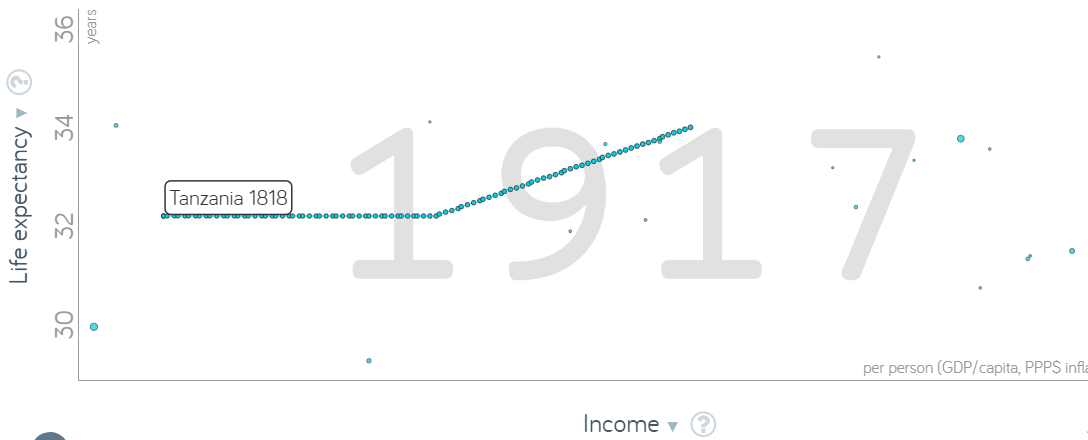
\includegraphics[width=0.49\linewidth ,  height=0.37\linewidth]{tanz_1917}
	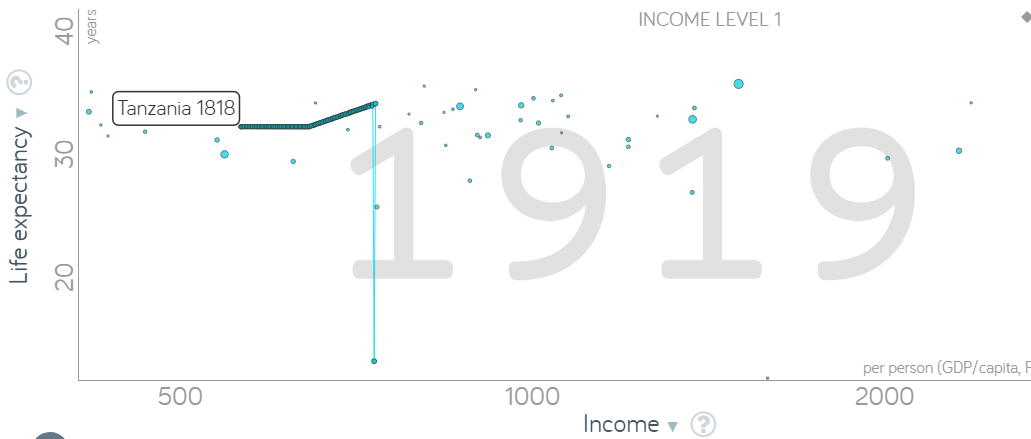
\includegraphics[width=0.49\linewidth , height=0.37\linewidth]{tanz_1919}
	\caption{Tanzanian Flu Epidemic}
	 \label{fig:tanz1917}
\end{figure}


 \begin{figure}[h!]
 \begin{center}
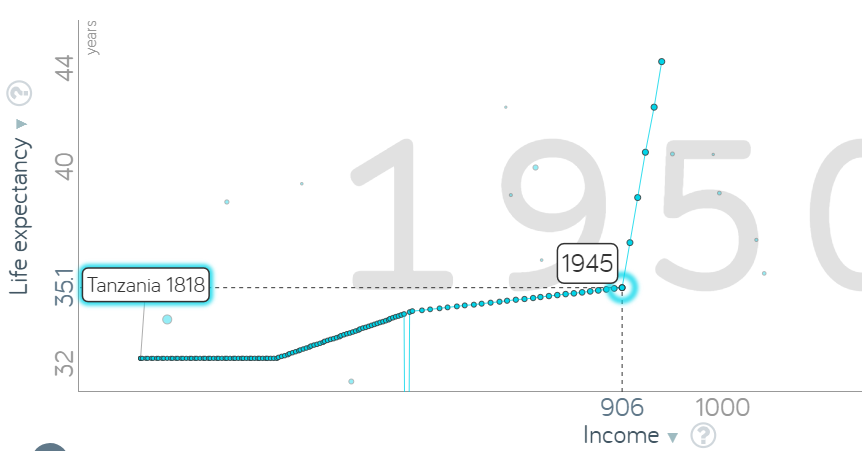
\includegraphics[width=0.59\linewidth]{tanz_late40s.png}
\caption{Effect of Trusteeship in the late 1940s}
 \label{fig:late40}
 \end{center}
 \end{figure}  
  
      \begin{figure}[h!]
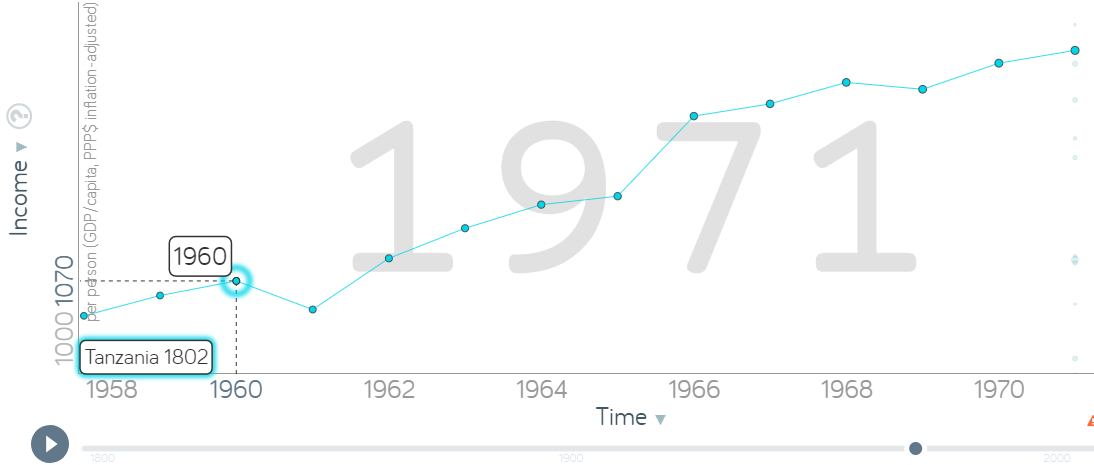
\includegraphics[width=\linewidth, height = 0.37\linewidth]{tanz_1960s_inc.png}
\caption{Tanzanian Independence}
 \label{fig:tanz60s}
 \end{figure}  


      \begin{figure}[h!]
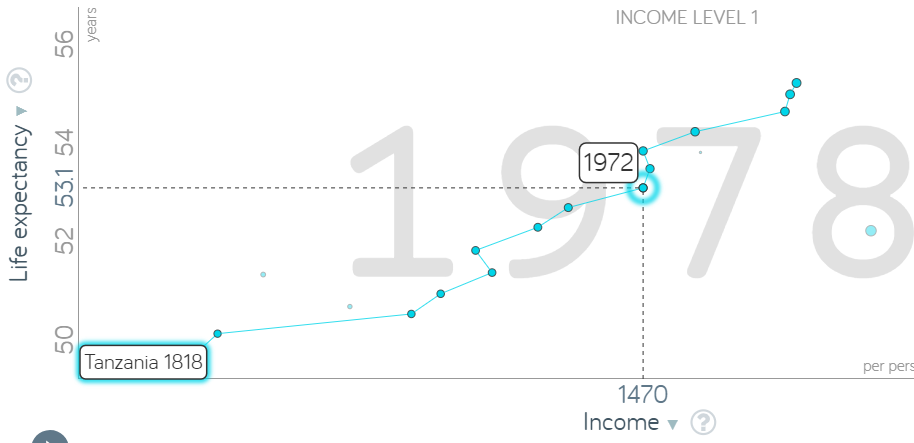
\includegraphics[width=\linewidth , height = 0.37\linewidth]{tanz_1970s.png}
\caption{OPEC Crisis}
 \label{fig:tanz70s}
 \end{figure}
 
     
\begin{figure}[h!]
	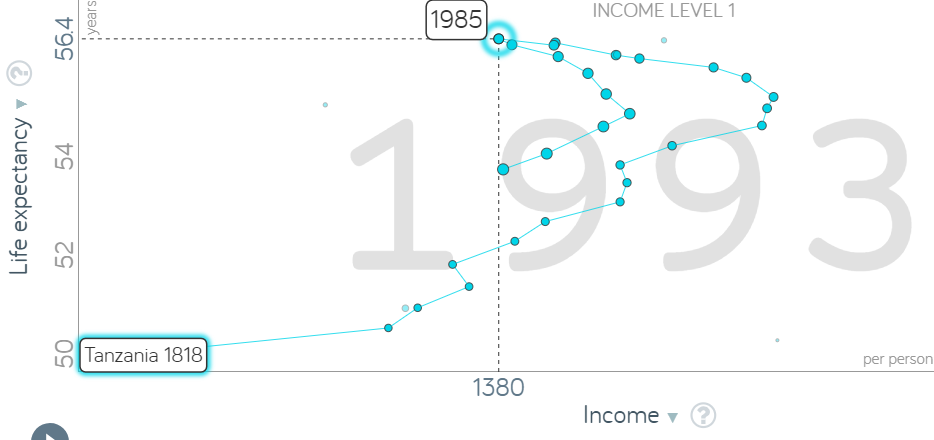
\includegraphics[width=0.49\linewidth ,  height=0.37\linewidth]{tanz_1980s}
	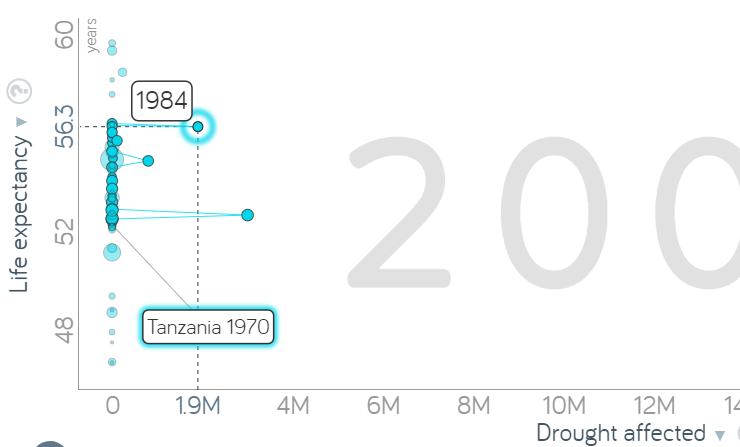
\includegraphics[width=0.49\linewidth , height=0.37\linewidth]{tanz_drought}
	\caption{Drought in the 1980s}
	 \label{fig:drought}
\end{figure}

 

 
\end{document}



\section{Dates}
\begin{itemize}
\item 1918
	\subitem flu epidemic see \ref{fig:tanz1917} and \ref{fig:tanz1918} see \ref{fig:tanz1919} see \ref{fig:tanz1918trail}. It went from 34 to 13.2 to 34.1. 
\item 1945-1950
	\subitem baby boom after WWII? Went from 35.1 (1945) to 44.3 (1950) with little to no change in income. See 		           Figure \ref{fig:late40s}

\item 1950-1951
	\subitem income per capita rose from 942 to 1040 in 1 year a 10.4\% increase. Unclear? End of Groundnut Scheme?
\item Union with Zanzibar did not seem to have a majr effect in 1964
\item Independence in 1961 had a major effect launching period of good times 
\item 1966
	\subitem 1 year after the union with zanzibar there was a 10\% increase in income per capita from 1190 to 1310. 
\item Could approach from a broader perspective. 1950-1970 was time of economic prosperity. With Tanganyikan independence and the introdcution of zanzibar. However it was based on import substitution. Really from 1960 on, 
	
\end{itemize}


https://atlas.media.mit.edu/en/profile/country/tza/

https://www.washingtonpost.com/archive/politics/1977/04/27/kenya-tanzania-border-tension-rises/3d85043b-bddb-4aaa-8265-659c40b56ec6/?noredirect=on&utm_term=.91b1268246ae


http://archive.unu.edu/unupress/unupbooks/uu34ee/uu34ee0i.htm#introduction

http://www.academicjournals.org/app/webroot/article/article1379789169_Ngowi.pdf

https://www.researchgate.net/publication/228625654_Economic_development_and_change_in_Tanzania_since_independence_The_political_leadership_factor

http://documents.worldbank.org/curated/en/649601468765032908/pdf/multi0page.pdf

https://www.imf.org/external/pubs/ft/fandd/2000/06/pdf/kanaan.pdf

https://www.fastonline.org/CD3WD_40/HDLHTML/EDUCRES/DEP18E/EN/CH04.HTM

https://www.britannica.com/place/Tanzania/History#ref281829

http://documents.worldbank.org/curated/en/747021468116373312/pdf/multi0page.pdf
